\section{Stable Diffusion (Latent Diffusion Model)}
\label{sec:stable_diffusion}


\begin{figure}
    \centering
    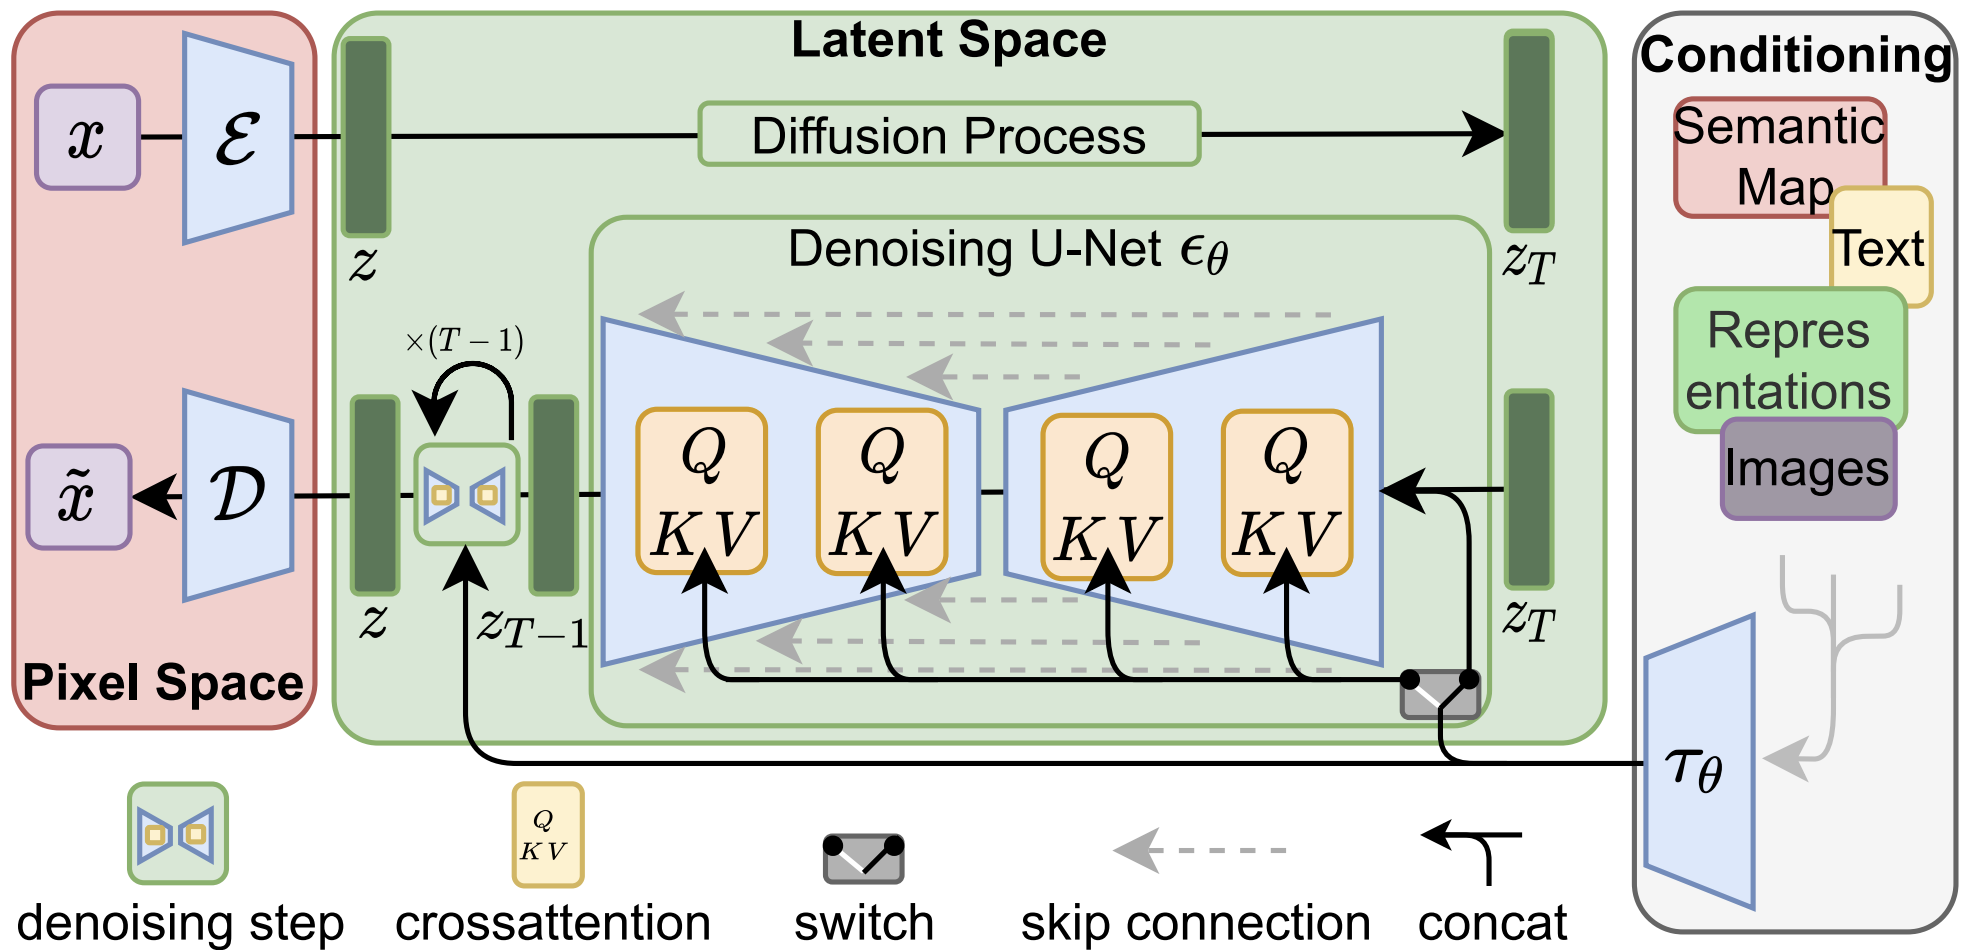
\includegraphics[width=0.6\textwidth]{images/diffusion_models/stable_diffusion/stable_diffusion.png}
    \caption{Stable diffusion scales better compared to other models \cite{stable_diffusion} (DALL-E, VQ-GAN) with less downsampling blocks ($f = 4$ instead of 16 as needed by VQ-GAN).}
\end{figure}


In the Stable Diffusion paper \cite{stable_diffusion} the authors suggested that computing gradients directly in DDPMs on the pixel space is inefficient, since this space is highly-dimensional and includes undesired high-frequency details. They suggest to convert the input images to a lower-dimensional latent representations and then apply the diffusion processes. The authors showed that this approach \textbf{scales better} and is more compute efficient \footnote{In the Stable Diffusion paper \cite{stable_diffusion} the authors showed that the model can be trained on a single GPU with 16GB of memory on images of $256\times 256$ resolution using CelebA-HQ dataset with 30 diffusion steps.} compared to working in pixel space. Moreover, the authors introduced general purpose \textbf{conditioning mechanism based on cross-attention} which allows multi-modal training.

A 2021 paper released by OpenAI \cite{openai_diffusion_beats_gans} shows that \textbf{diffusion models can outperform GANs} in terms of image fidelity by trading off diversity.











\subsection{The U-Net backbone}
\label{subsec:stable_diffusion_u_net_backbone}

U-Net (first introduced in 2015) \cite{unet} is a convolutional neural network (CNN) architecture that is commonly used in diffusion models. U-Net is used as a backbone for denoising the latent variables $z_1, ..., z_T$. The U-Net architecture is a symmetric encoder-decoder network with skip connections between the encoder and decoder: the skip connections help the network to learn better by minimizing the \textbf{exploding / vanishing gradient problems} \cite{exploding_vanishing_gradients}.

\begin{figure}
    \centering
    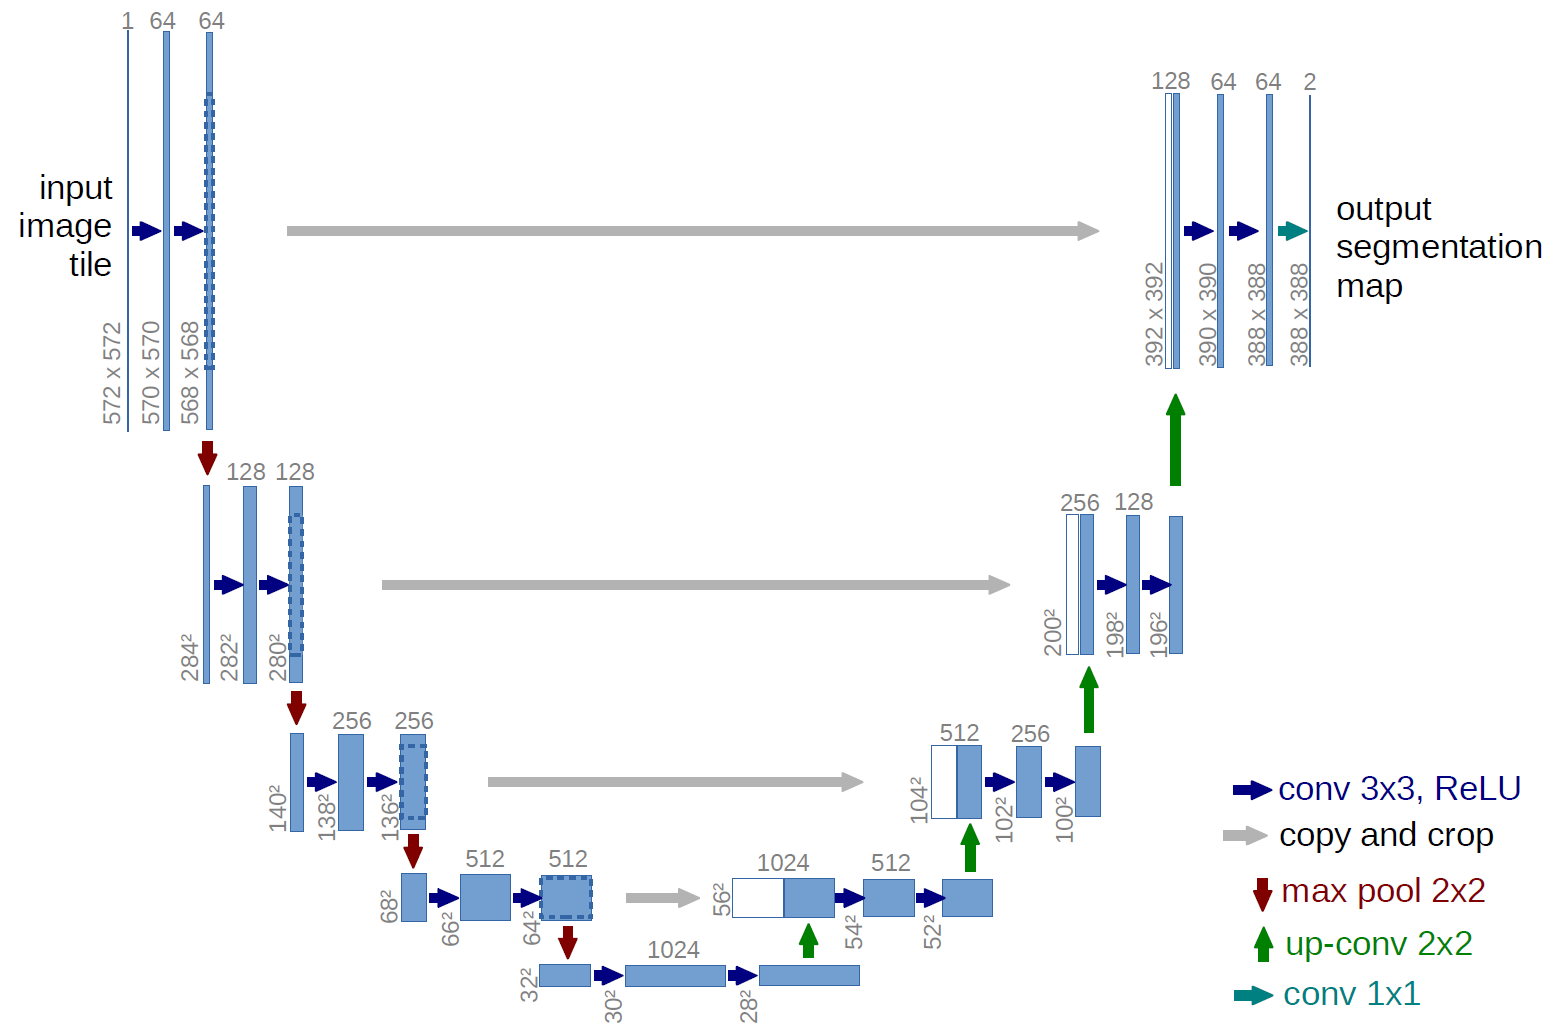
\includegraphics[width=0.5\textwidth]{images/diffusion_models/stable_diffusion/u-net-architecture.png}
    \caption{The U-Net architecture \cite{unet} with convolutional and deconvolutional layers \& skip connections.}
    \label{fig:unet_architecture}
\end{figure}

In figure \ref{fig:unet_architecture} the U-Net is shaped like a 'U' in which the input is downsampled to low spatial resolution and high feature channels and then upsampled back again. The convolution kernel size is 3x3 and they use ReLU activation function.








\subsection{Sinusoidal embeddings}
\label{subsec:sinusoidal_embeddings}

The diffusion process uses \textbf{timestep embeddings} which is the embeddings representing the current diffusion timestep: $t \in [0, T]$. Instead of directly using timestep scalar, we first convert it to embeddings. This way the model knows if it is in the beginning of the diffusion or at the later stages, which is essential for removing noise (because noise schedulers depend on the current timestep).

To get the embeddings, the timestep is first projected into a \textbf{sinusoidal embedding}, similar to the way positional encodings are used in transformers.

\begin{figure}[h]
    \centering
    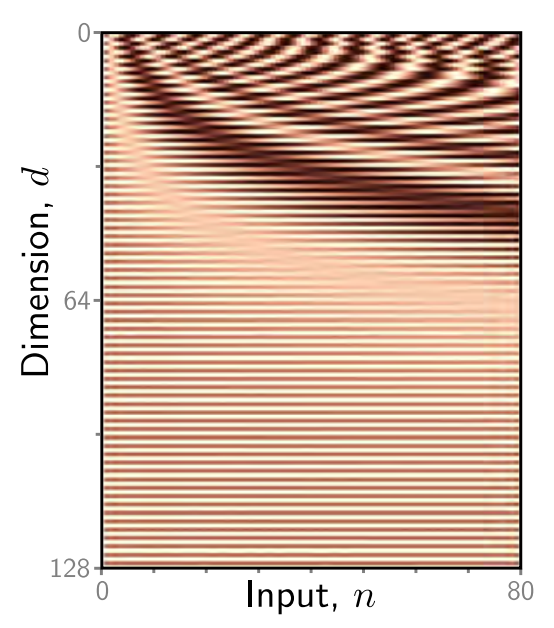
\includegraphics[width=0.25\textwidth]{images/diffusion_models/stable_diffusion/positional_encodings.png}
    \caption{Sinusoidal positional embeddings used in a transformers \cite{understanding_deep_learning_book_2024}. \textit{X axis}: the input scalar (position in a transformer or timestep in diffusion model). \textit{Y axis}: the embeddings dimensions \cite{understanding_deep_learning_book_2024}.}
    \label{fig:sinusoidal_embeddings}
\end{figure}

In figure \ref{fig:sinusoidal_embeddings} we can see the sinusoidal positional embeddings used in a transformer model, which is similar to timestep embeddings. The pattern is sinusoidal where lighter regions indicate lower values and darker regions indicate higher values. Each column in the X axis is a \textbf{unique embedding}. For example, the scalar '1' will have different encodings than a scalar '2', which helps distinguish the position / timestep of the input sequence.

\begin{lstlisting}[language=Python, breaklines=true, caption={Timestep embeddings in Stable Diffusion: we convert the timestep to an embedding.}, label={lst:timestep_embeddings_stable_diffusion}]
def get_time_embedding(timestep):
    # Shape: (160,)
    freqs = torch.pow(10000, -torch.arange(start=0, end=160, dtype=torch.float32) / 160) 
    # Shape: (1, 160)
    x = torch.tensor([timestep], dtype=torch.float32)[:, None] * freqs[None]
    # Shape: (1, 160 * 2)
    return torch.cat([torch.cos(x), torch.sin(x)], dim=-1)
\end{lstlisting}

The general formula for timestep embeddings is given in equation \ref{eq:timestep_embeddings}. The code snippet in listing \ref{lst:timestep_embeddings_stable_diffusion} is taken from \href{https://github.com/hkproj/pytorch-stable-diffusion/blob/e0cb06de011787cdf13eed7b4287ad8410491149/sd/pipeline.py#L164}{a re-implementation of Stable Diffusion}.

\begin{equation}
    \text{Enc}_i(t) =
    \begin{cases}
        \sin\left(\frac{t}{10000^{\frac{2i}{d}}}\right) & \text{if } i \text{ is even} \\
        \cos\left(\frac{t}{10000^{\frac{2i}{d}}}\right) & \text{if } i \text{ is odd}
    \end{cases}
    \label{eq:timestep_embeddings}
\end{equation}










\subsection{Architecture}

\begin{figure}
    \centering
    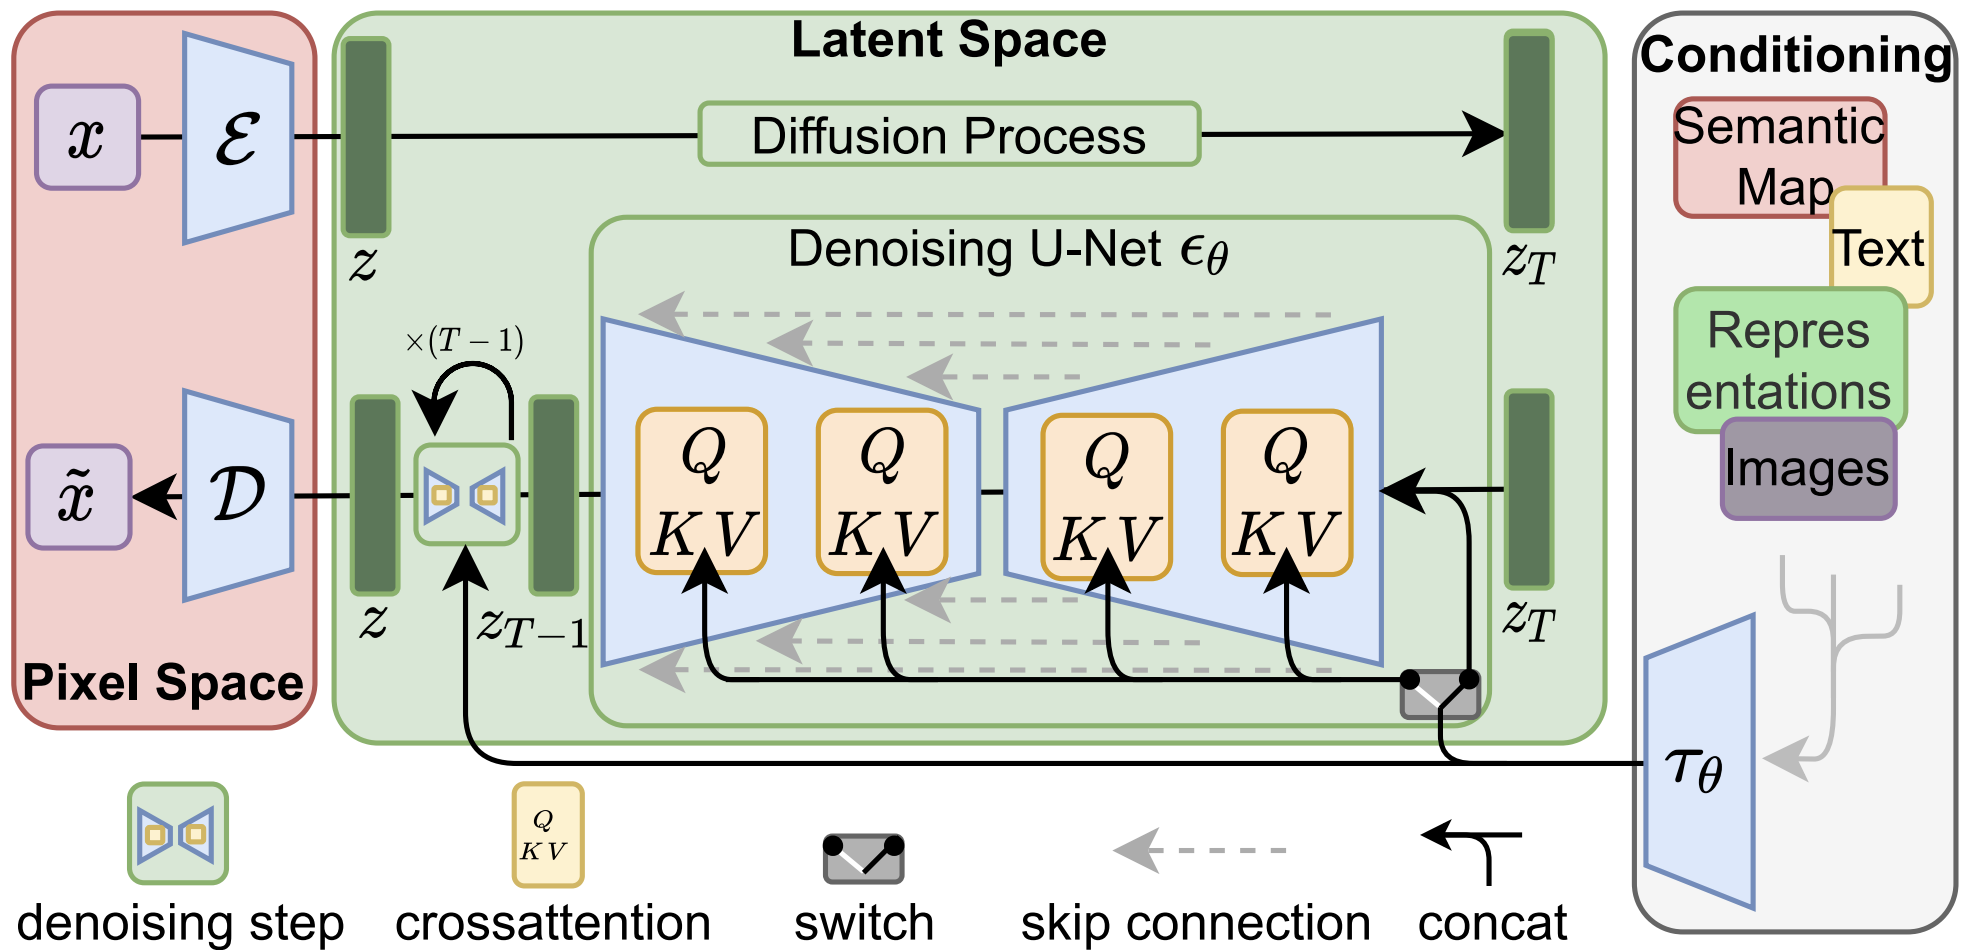
\includegraphics[width=0.5\textwidth]{images/diffusion_models/stable_diffusion/architecture.png}
    \caption{Stable Diffusion architecture \cite{stable_diffusion}.}
    \label{fig:stable_diffusion_architecture}
\end{figure}

The high-level architecture is shown in figure \ref{fig:stable_diffusion_architecture}. The stable diffusion model, which is a latent diffusion model (LDM), consists of: 

\begin{itemize}
    \item Variational autoencoder (VAE) which compresses the input images into regularized latent space. It consists of:
    \begin{itemize}
        \item Encoder $\varepsilon$ which converts the input images $x$ to latent space $z$.
        \item Decoder $\mathcal{D}$ which converts the latent vector $z$ back to the pixel space $\tilde{x}$.
    \end{itemize}
    \item A U-Net backbone which serves as the noise prediction network, predicts the noise needed to denoise the intermediate latent vectors $z_T, ..., z_1$ in each step. It incorporates timestep embeddings as an essential input.
    \item A domain specific encoder $\tau_\theta$ which encodes the conditional information (text prompts, images, segmentation masks) into tokens which will be used in the cross-attention layers, or concatenated with the latent vector (the switch mechanism).
\end{itemize}







\subsection{Conditioning}

Cross-attention (appendix \ref{appendix:attention}) is used in Stable Diffusion for \textbf{multi-modal conditioning}: it guides the model to output images based on conditional information. Although this information is multi-modal (e.g. images, text, segmentation masks), the cross-attention layers in the U-Net and the switch mechanism able to process them all.

\textbf{Text conditioning}: if the conditioning signal is text prompt, the domain specific encoder $\tau_\theta$ is a text encoder (tokenizer) which converts the text words to embeddings (tokens). In the paper \cite{stable_diffusion} the authors used a \href{https://github.com/CompVis/latent-diffusion/blob/a506df5756472e2ebaf9078affdde2c4f1502cd4/ldm/modules/encoders/modules.py#L138}{\textbf{frozen CLIPTokenizer}}, which is a pre-trained tokenizer trained on specific vocabulary, and special tokens (beginning of sentence, end of sentence, padding, mask tokens and more). However, digging into the source code, you will find other text encoders as well such as \href{https://github.com/CompVis/latent-diffusion/blame/a506df5756472e2ebaf9078affdde2c4f1502cd4/ldm/modules/encoders/modules.py#L53}{\textbf{BERT}} \cite{bert}.

\textbf{Switch mechanism}: In figure \ref{fig:stable_diffusion_architecture} the 'switch' in the diagram is used for different kinds of conditional information. If the conditional information is spatial (such as images, layouts, semantic masks), they use concatenation with $z_T$. In the case of text (not spatial), they use cross-attention layers. 

We dive deeper into self-attention, multi-head attention and cross-attention in the appendix \ref{appendix:attention}, which are commonly used in other image and video synthesis models.













\subsection{Classifier-free diffusion guidance (CFG)}

\label{subsec:classifier_free_diffusion_guidance}

Classifier-free guidance (CFG) is used in Stable Diffusion to control the influence of the conditioning signal and balance between being faithful to the conditioning signal or being diverse in the generated samples.

So far we have focused on modeling just the data distribution $p(x)$. However, we are often also interested in learning conditional distribution $p(x|y)$, which would enable us to explicitly control the data we generate through conditioning signal $y$.

We can add conditioning information alongside the timestep information, at each iteration (appendix B equation 8 of \cite{ddpm}, appendix H equation 31 of \cite{openai_diffusion_beats_gans}):

\[
p(x_{0:T}) = p(x_T) \prod_{t=1}^{T} p_\theta (x_{t-1} | x_{t, y})
\]

where $p$ is the reverse diffusion process that removes noise in image $x_t$ in steps $t = T, T-1, ..., 0$, $y$ is the conditioning information

When training a diffusion model to generate images based on specific conditional information, there's a risk that the model might not fully consider or even ignore these conditions, using this vanilla formulation. To address this, a technique called "guidance" is used. Guidance allows us to explicitly control \textbf{how much influence the conditions have on the generated images}, but this can sometimes lead to less variety in the results. In other words, we use weight to control how much the model should pay attention to the conditioning signal.


Conditioning a generative model can be achieved through two methods: 

\begin{itemize}
    \item classifier guidance
    \item and classifier-free guidance.
\end{itemize}





\subsubsection*{Classifier guidance}

Classifier guidance \cite{openai_diffusion_beats_gans} involves \textbf{training a separate model} to condition the output, and is based on score-based diffusion models \cite{score_based_generative_modeling}. 

Classifier guidance formulation is given as:

\[
\nabla \log p(x_t | y) = \underbrace{\nabla \log p(x_t)}_{\text{unconditional score}} + \underbrace{\gamma \nabla \log p(y | x_t)}_{\text{adversarial gradient}}
\]

where $\gamma$ is a hyperparameter that controls the strength of the conditioning signal in classifier guidance method.








\subsubsection*{Classifier-free guidance}

In Classifier-free guidance (CFG) \cite{classifier_free_guidance}, instead of training two networks, one conditional network and an unconditional network, we train a single network, and during training, \textbf{we set the conditioning signal to zero} with some probability. This way, the network becomes a mix of conditioned and unconditioned networks, and we can take the conditioned and unconditioned output and combine them with weight that indicates how much we want the network to pay attention to the conditioning signal. 

The formulation for classifier-free guidance is given by:

\[
\nabla \log p(x_t | y) = \underbrace{\gamma \nabla \log p(x_t | y)}_{\text{conditional score}} + \underbrace{(1 - \gamma) \nabla \log p(x_t)}_{\text{unconditional score}}
\]

In contrast to classifier guidance, classifier-free guidance streamlines the training process and lowers computational costs by utilizing a single model instead of training two separate models.

\begin{lstlisting}[language=Python, caption={Classifier-free guidance (CFG) in Stable Diffusion.}, label={lst:cfg_stable_diffusion}]
if do_cfg:
    output_cond, output_uncond = model_output.chunk(2)
    model_output = cfg_scale * (output_cond - output_uncond) + output_uncond
\end{lstlisting}

In listing \ref{lst:cfg_stable_diffusion} the code snippet is taken from \href{https://github.com/hkproj/pytorch-stable-diffusion/blob/e0cb06de011787cdf13eed7b4287ad8410491149/sd/pipeline.py#L135C1-L136C1}{a re-implementation of Stable Diffusion}, but the official implementation of Stable Diffusion is \href{https://github.com/CompVis/stable-diffusion/blob/21f890f9da3cfbeaba8e2ac3c425ee9e998d5229/ldm/models/diffusion/ddim.py#L178C1-L179C1}{very similar}.

















\subsection{Contrastive Language Image Pre-training (CLIP)}
\label{subsec:clip}

In Stable Diffusion, the authors used CLIP as the text encoder for the conditional text prompts.

CLIP (Contrastive Language Image Pre-training) \cite{openai_clip} is a model developed by OpenAI that learns visual concepts from text supervision. The model builds \textbf{associations between images and text prompts}. Often this association is called 'text-image alignment', or 'image-text alignment'. It models how well a generated image corresponds to its associated text description.

The \textbf{CLIPTokenizer}, which is part of the CLIP model, converts text prompts to a sequence of tokens which are then used in the latent space of the Stable Diffusion model.

\begin{figure}
    \centering
    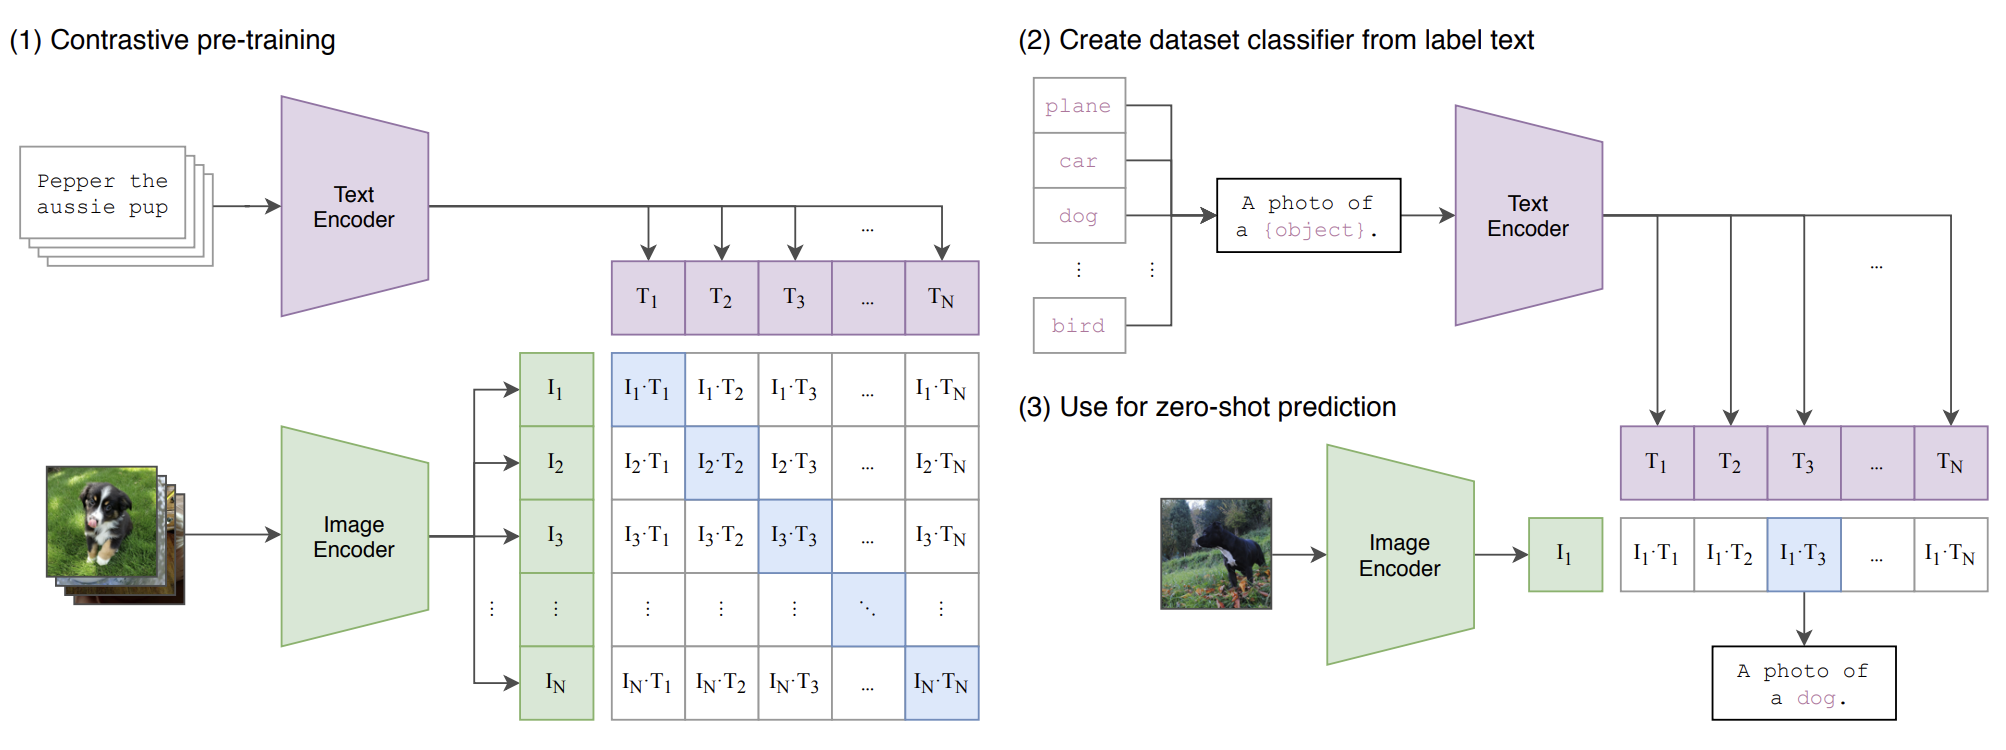
\includegraphics[width=0.7\textwidth]{images/diffusion_models/stable_diffusion/clip.png}
    \caption{(1) Contrastive pre-training stage of a CLIP model (training stage). (2) and (3): after the model has been pre-trained, its used as a zero-shot image classifier \cite{openai_clip}.}
    \label{fig:openai_clip}
\end{figure}

In figure \ref{fig:openai_clip},  $I_1, ..., I_N$ are the images, and $T_1, ..., T_N$ are the text prompts. The output is a \textbf{matrix of similarity scores} between the images and the text descriptions. Ideally in the matrix diagonal we get high similarity score (1) indicating high text-image alignment, and all other entries ideally should have low similarity score (0), indicating mismatch in text-image alignment.

The CLIP network is compromised of:

\begin{itemize}
    \item \textbf{Image encoder}: converts images to image embeddings.Its typically a vision transformer (ViT) \cite{vision_transformer} (appendix \ref{appendix:vision_transformer}) or a ResNet \cite{resnet} model.
    \item \textbf{Text encoder}: converts text descriptions to text embeddings. Its typically implemented as a transformer, or less common as a continuous bag of words \cite{cbow_word2vec} (known as Word2Vec model by Google, 2013 \cite{cbow_word2vec}).
    \item \textbf{Training objective}: the CLIP model is trained using a contrastive objective (commonly referred to as CLIP objective), where the goal is to minimize the cosine distance in the main diagonal and maximize the distance for non-matching image-text pairs (off diagonal).
\end{itemize}





















\subsection{DDIM Sampler}
\label{subsec:ddim_sampler}

\begin{figure}[ht]
    \centering
    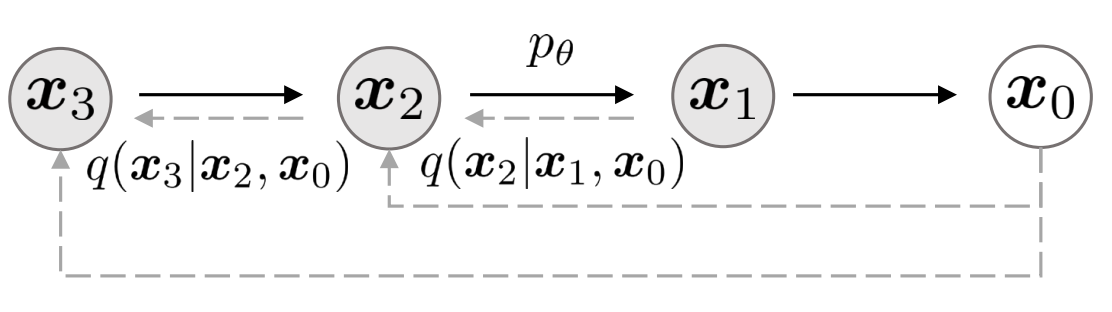
\includegraphics[width=0.4\textwidth]{images/diffusion_models/stable_diffusion/ddim_non_markov_process.png}
    \caption{Non-Markovian inference in DDIM. Each step depends on both the previous step and the initial state $x_0$ \cite{ddim}.}
    \label{fig:ddim_non_markov_process}
\end{figure}

Denoising Diffusion Implicit Models (DDIM), introduced in \cite{ddim}, provide an \textbf{efficient sampling method} for diffusion models, offering improvements over the traditional Denoising Diffusion Probabilistic Models (DDPM) \cite{ddpm}. Unlike DDPM sampler, which uses a fixed noise schedule and stochastic sampling, DDIM introduces a flexible noise schedule and a \textbf{deterministic sampling process}, enabling faster inference (10x to 50x speedup compared to DDPM \cite{ddim}).

Key points \& main contributions of the DDIM paper:

\begin{itemize}
    \item \textbf{Non-Markovian process}: As illustrated in figure \ref{fig:ddim_non_markov_process}, DDIM's reverse process depends on both the previous step and the initial state $x_0$, forming a deterministic trajectory through the latent space.
    \item \textbf{Implicit probabilistic model}: DDIM is an implicit probabilistic model, meaning that it doesn't directly model the joint distribution of the data but rather models the conditional distribution of the data given the noise.
    \item \textbf{Deterministic sampling}: Noise is removed directly in a controlled manner, skipping unnecessary diffusion steps and avoiding stochasticity.
    \item \textbf{Training objective}: DDIM uses the same training objective as DDPM and no modifications are needed.
    \item \textbf{Sampling process}: Sampling in DDIM involves sampling from the prior distribution and then iteratively sampling from the conditional distributions. This process is faster than traditional diffusion models because it doesn't require simulating the entire Markov chain.
\end{itemize}

DDIM introduces a generalized forward process:

\[
q_\sigma (x_{t-1} | x_t, x_0) = \mathcal{N} \left( \sqrt{\alpha_{t-1}} x_0 + \sqrt{1 - \alpha_{t-1} - \sigma_t^2} \cdot \frac{x_t - \sqrt{\alpha_t} x_0}{\sqrt{1 - \alpha_t}}, \sigma_t^2 I \right)
\]

where $\sigma \in \mathbb{R}^T_{\geq 0}$ controls the stochasticity of the forward process. When $\sigma \rightarrow 0$, the process becomes fully deterministic, as $x_{t-1}$ is uniquely determined by $x_t$ and $x_0$.

\begin{figure}
    \centering
    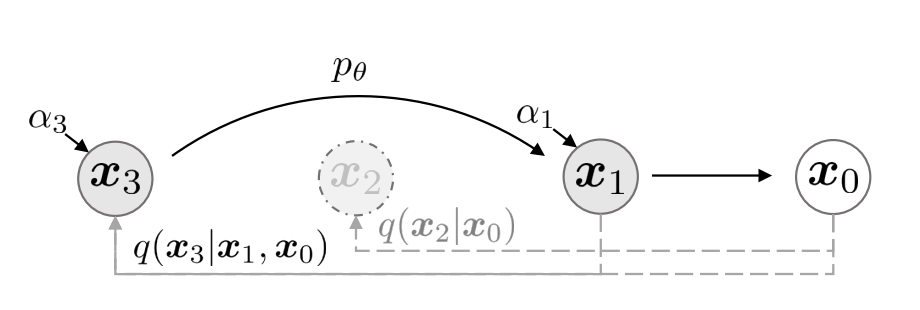
\includegraphics[width=0.5\textwidth]{images/diffusion_models/stable_diffusion/ddim_sampling_process.png}
    \caption{DDIM sampling \cite{ddim}. In the figure, $x_3$ depends only on $x_0$ and $x_1$ (and not $x_2$). This process can be generalized to all subsets of steps.}
    \label{fig:ddim_sampling_process}
\end{figure}

\begin{figure}
    \centering
    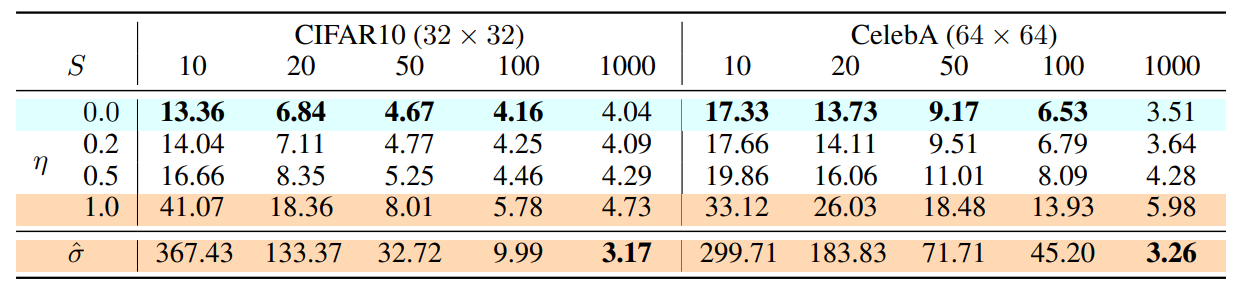
\includegraphics[width=0.7\textwidth]{images/diffusion_models/stable_diffusion/ddim_sample_quality.png}
    \caption{DDIM gives almost the same sample quality compared to DDPM sampler, and requires less compute since we skip some of the diffusion steps. The stochasticity of the model is controlled by $\eta$ \cite{ddim}.}
    \label{fig:ddim_sample_quality}
\end{figure}

In figure \ref{fig:ddim_sample_quality} DDIM gives almost the same sample quality in FID metric (equation \ref{eq:fid_score}, lower is better) compared to DDPM and require much less compute. The experiment was done on CIFAR10 and CelebA datasets, with 10,20,50,100,1000 steps. When $\eta = 0$ (blue) the model is deterministic (DDIM process), and when $\eta = 1$ (orange) the model is stochastic (DDPM process).















\subsection{Training}

Stable Diffusion is trained in CFG manner (section \ref{subsec:classifier_free_diffusion_guidance}).

The authors made simplified loss objective which predicts the noise removal process at each step:

\[
    L_{\text{DM}} = \mathbb{E}_{x, \epsilon \sim \mathcal{N} (0, 1), t} \left[ \Vert \epsilon - \epsilon_\theta(x_t, t) \Vert _2^2 \right]
\]

This loss function is similar to the loss function of DDPM (equation \ref{eq:ddpm_loss}).













\subsection{Implementation of $\tau_\theta$ transformer for conditional LDMs}

The researchers provded high level overview of the implementation of the conditional encoder for text $\tau_\theta$, consisted of $N$ transformer blocks (appendix E.2 of \cite{stable_diffusion}):

\begin{align*}
    &\zeta \leftarrow \text{TokEmb}(y) + \text{PosEmb}(y) \\
    &\text{for } i = 1, \ldots, N : \\
        &\hspace{1cm} \zeta_1 \leftarrow \text{LayerNorm}(\zeta) \\
        &\hspace{1cm} \zeta_2 \leftarrow \text{MultiHeadSelfAttention}(\zeta_1) + \zeta \\
        &\hspace{1cm} \zeta_3 \leftarrow \text{LayerNorm}(\zeta_2) \\
        &\hspace{1cm} \zeta \leftarrow \text{MLP}(\zeta_3) + \zeta_2 \\
    &\zeta \leftarrow \text{LayerNorm}(\zeta)
\end{align*}

where:

\begin{itemize}
    \item $\zeta := \tau_\theta(y)$ is the unmasked transformer output (the transformer processes the tokenized version of $y$), which is then used in the cross-attention mechanism of the stable diffusion model.
    \item TokEmb is the token embeddings.
    \item PosEmb is the positional embeddings.
    \item LayerNorm is the layer normalization (appendix \ref{appendix:blocks_norm}).
    \item MultiHeadSelfAttention is the multi-head self-attention mechanism (appendix \ref{appendix:attention}).
    \item and MLP is the multi-layer perceptron (appendix \ref{appendix:blocks}) block.
\end{itemize}


\begin{figure}[h]
    \centering
    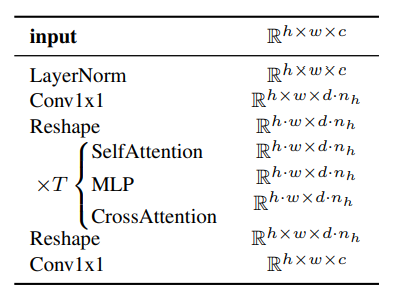
\includegraphics[width=0.3\textwidth]{images/diffusion_models/stable_diffusion/transformer_block.png}
    \caption{Architecture of the transformer block used in Stable Diffusion, where $n_h$ denotes the number of attention heads and $d$ the dimensionality per head \cite{stable_diffusion}.}
\end{figure}











\subsection{Details on Autoencoders Models}

In the stable diffusion paper, the researchers trained the pixel-space encoder $\varepsilon$ and the decoder $\mathcal{D}$ in adversarial manner (adversarial loss \cite{vqgan}). A patch-based discriminator $D_\psi$ is optimized to differentiate the original image from reconstructed image $\mathcal{D} (\varepsilon (x))$ which helps guide the autoencoder.

In addition, the researchers used two methods for regularizing the latent space:

\begin{itemize}
    \item \textbf{KL-divergence regularization}: similar to VAEs where the latent space is a distribution, the KL regularization objective pushes the latent space to be close to a standard normal distribution.
    \item \textbf{VQ regularization}: similar to VQ-GAN and VQ-VAE (sections \ref{vqgan} and \ref{vqvae}), the vector quantization regularization forces the latent space to be discrete, which can help the model to learn better by using a codebook $\mathcal{Z}$.
\end{itemize}

They factorized the KL term by a factor of $\sim 10^{-6}$, and in VQ regularization they used a big codebook.

The full loss objective to train the autoencoder model $(\varepsilon, \mathcal{D})$ is given by:

\begin{equation*}
    L_{\text{Autoencoder}} = \min_{\varepsilon, \mathcal{D}} \max_{\psi} \left( L_{\text{rec}} (x, \mathcal{D} (\varepsilon (x))) - L_{\text{adv}} (\mathcal{D} \varepsilon (x)) + \log \mathcal{D}_\psi (x) + L_{\text{reg}} (x; \varepsilon, \mathcal{D}) \right)
\end{equation*}


















\subsection{Experiments}

The researchers conducted several experiments with different LDM downsampling factors, and compared the results with other state-of-the-art models (DALL-E, VQGAN, StyleGAN, ProjectedGAN, CogView, GLIDE, and others).

\begin{figure}
    \centering
    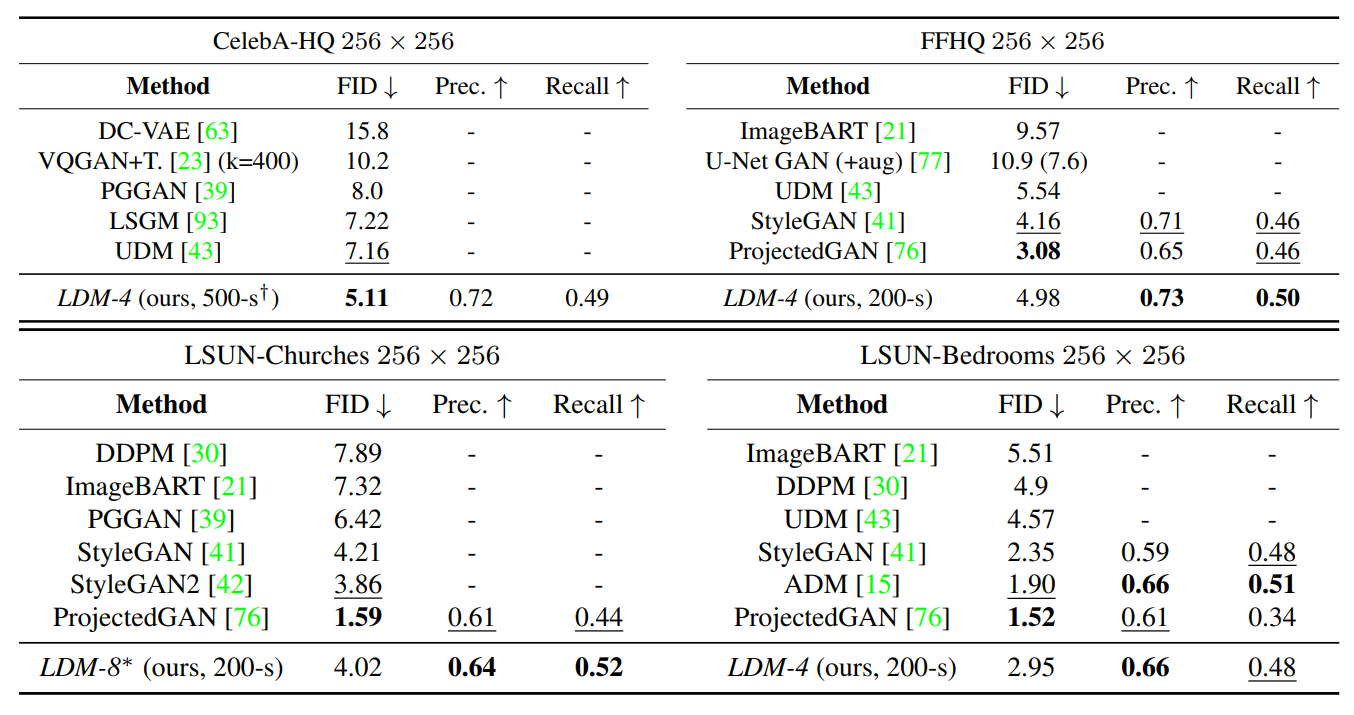
\includegraphics[width=0.7\textwidth]{images/diffusion_models/stable_diffusion/experiments_1.png}
    \caption{Unconditional image synthesis evaluation between LDM (Stable Diffusion) and other models across 4 datasets \cite{stable_diffusion}.}
    \label{fig:stable_diffusion_experiments_unconditional}
\end{figure}

In figure \ref{fig:stable_diffusion_experiments_unconditional} we clearly see that LDM outperforms most of the state-of-the-art models, across multiple metrics and datasets. $\dagger$ refers to the DDIM sampler steps (500 top-left, 200 top-right, 200 bottom-left, 200 bottom-right).

\begin{figure}
    \centering
    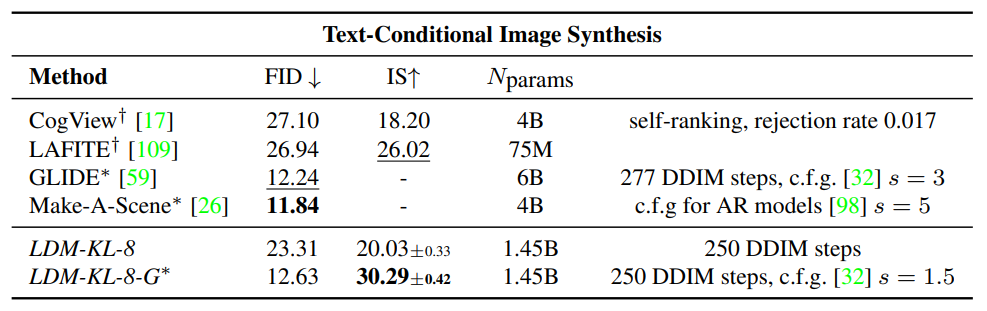
\includegraphics[width=0.6\textwidth]{images/diffusion_models/stable_diffusion/experiments_2.png}
    \caption{Evaluation of text-conditioned image synthesis on MS-COCO dataset. LDM with 250-DDIM steps is on par with the most recent diffusion and autoregressive methods, \textbf{while using significantly less parameters} (1.45 billion) \cite{stable_diffusion}.}
\end{figure}

For text-to-image tasks, the researchers trained a 1.45B parameters model conditioned on language prompts on LAION-400M dataset. The model uses \textbf{BERT-Tokenizer} \footnote{Its important to note that the researchers used the BERT text tokenizer in the paper, however, in the \href{https://github.com/CompVis/latent-diffusion}{offical released implementation of Stable Diffusion} they used CLIP tokenizer. The reason is that in the Imagen paper \cite{imagen}, the researchers found out that using larger language models had more impact on generated image quality than larger image generation components. This fact is shown in figure \ref{fig:imagen_clip_score_bigger_llm}.} \cite{bert} and implement $\tau_\theta$ (the domain-specific conditional encoder) as a transformer.

\begin{figure}
    \centering
    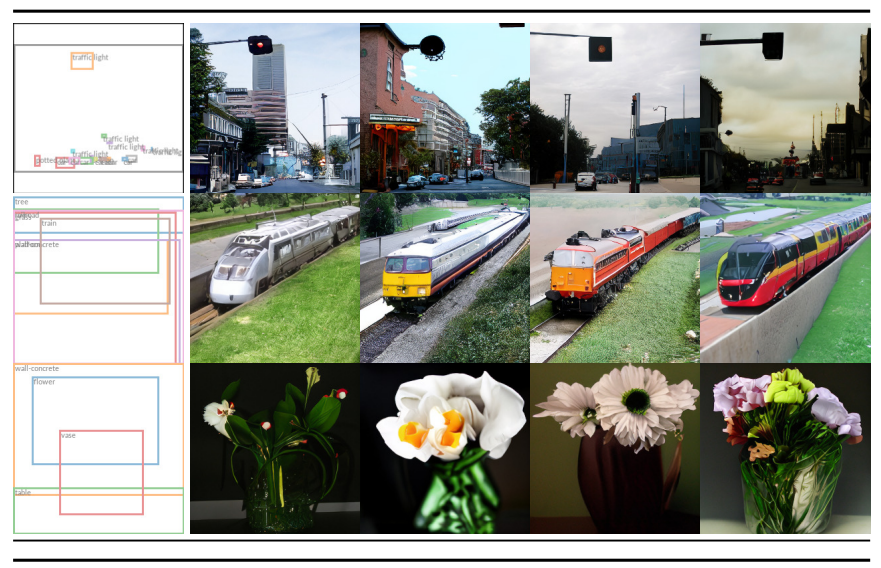
\includegraphics[width=0.5\textwidth]{images/diffusion_models/stable_diffusion/experiments_3.png}
    \caption{Samples of Stable Diffusion conditioned on semantic layouts \cite{stable_diffusion}.}
    \label{fig:stable_diffusion_experiments_semantic_layouts}
\end{figure}

For semantic layouts, the model is trained to synthesis images based on semantic layouts from the OpenImages dataset and fine-tuned on COCO dataset (figure \ref{fig:stable_diffusion_experiments_semantic_layouts}).

In figure \ref{fig:imagen_scaling_encoder_more_impactful_than_unet_scaling}, which is from Imagen paper \cite{imagen}, we see that using larger text encoder has more impact on image quality than larger image generation components (like the U-Net). This is why in Stable Diffusion, the implementation uses CLIP tokenizer instead of BERT tokenizer (which was originally used in the paper).
